\usetikzlibrary{datavisualization}
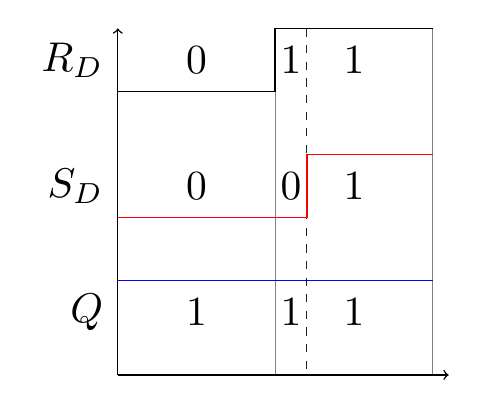
\begin{tikzpicture}[xscale=2, yscale=0.8]

\foreach \x in {1, 2}
    \draw[help lines] (\x, 1) -- (\x, -4.5);
\foreach \x/\l in {0.5/0, 1.1/1, 1.5/1}
    \node[scale=1.5] at (\x, 0.5) {$\l$};
\foreach \x/\l in {0.5/0, 1.1/0, 1.5/1}
    \node[scale=1.5] at (\x, -1.5) {$\l$};
\foreach \x/\l in {0.5/1, 1.1/1, 1.5/1}
    \node[scale=1.5] at (\x, -3.5) {$\l$};

\draw[dashed, green!20!black] (1.2, 1) -- (1.2, -4.5);

\draw[->] (0,-4.5) -- (2.1,-4.5);
\draw[->] (0,-4.5) -- (0,1);

\draw[->] (0,-4.5) -- (2.1,-4.5);
\draw[->] (0,-4.5) -- (0,1);

\datavisualization [
  xy Cartesian,
  visualize as line/.list={R,S,O},
  S={style={red}},
  O={style={blue}},
]
  data[set=R] {
    x, y
    0, 0
    1, 0
    1, 1
    2, 1
  }
  data[set=S] {
    x, y
    0, -2
    1.2, -2
    1.2, -1
    2, -1
  }
  data[set=O] {
    x, y
    0, -3
    2, -3
  }
  ;

  \node[left, scale=1.5] at (0,  0.5){$R_D$};
  \node[left, scale=1.5] at (0, -1.5){$S_D$};
  \node[left, scale=1.5] at (0, -3.5){$Q$};
\end{tikzpicture}